% Relaxation dispersion.
%%%%%%%%%%%%%%%%%%%%%%%%

\chapter[Relaxation dispersion]{The analysis of relaxation dispersion} \label{ch: relax-disp}
\index{relaxation dispersion|textbf}

\begin{figure*}[h]
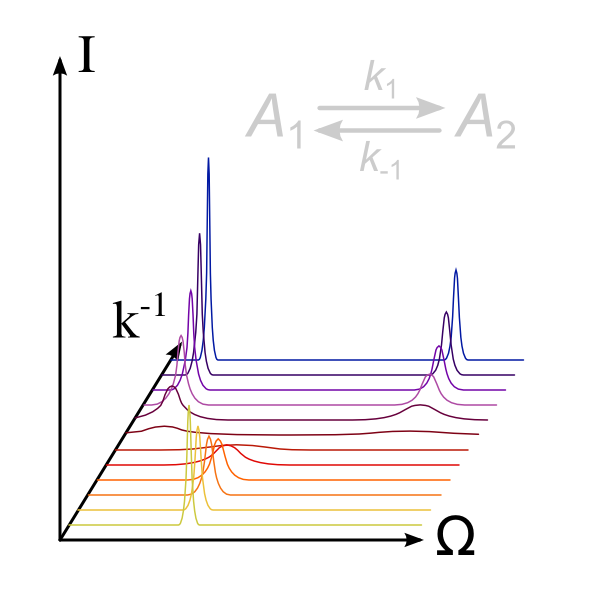
\includegraphics[width=5cm, bb=0 0 1701 1701]{graphics/analyses/relax_disp_600x600}
\end{figure*}


% Introduction.
%%%%%%%%%%%%%%%

\section{Introduction to relaxation dispersion}

Relaxation dispersion is the experimental modulation of chemical exchange relaxation.  For the $\Ronerho$-type experiment in which the nucleus of interest is spin-locked, either the spin-lock field strength or the offset between the spin-lock pulse and the chemical shift of the spins is used to modulate the exchange.  For the CPMG-type experiment, varying the time between the pulses modules the exchange.  Both experiment types are handled by relax.


% The models.
%%%%%%%%%%%%%

\section{The modelling of dispersion data}

For a system under the influence of chemical exchange, the evolution of the transverse magnetisation is given by the \citet{Bloch46} equations as modified by \citet{McConnell58} for chemical exchange -- the Bloch-McConnell equations.
For a two state exchange jumping between states A and B, the equation is:

\begin{equation} \label{eq: Bloch-McConnell}
    \frac{d}{dt} \left[ 
        \begin{array}{c}
            M_A^+(t) \\
            M_B^+(t)
        \end{array}
    \right] = \left[
        \begin{array}{cc}
            -i\Omega_A-\RtwozeroA-\pB\kex & \pA\kex \\
            \pB\kex & -i\Omega_B-\RtwozeroB-\pA\kex \\
        \end{array}
    \right] \left[
        \begin{array}{c}
            M_A^+(t) \\
            M_B^+(t)
        \end{array}
    \right] .
\end{equation}

The solution to this equation then Fourier transformed to produce the NMR spectrum.  However the analytic or closed-form frequency-domain solution remains intractable.

Solutions can nevertheless be found by either making assumptions or restrictions about the exchange process and then analytically solving~\ref{eq: Bloch-McConnell} or by numerical simulation.
The modelling of relaxation dispersion data can hence be catergorised into these two distinct methodologies:

\begin{description}
\item[Analytical models:]\index{relaxation dispersion!Analytical model}  Optimisation of models based on analytical, closed-form expressions derived from the Bloch-McConnell equations subject to certain conditions.
\item[Numerical models:]\index{relaxation dispersion!Numerical model}  Optimisation of models via numerical integration of the Bloch-McConnell equations.
\end{description}

Currently only the optimisation of the analytic models is supported in relax.
These models are dependant upon whether the data originates from a CPMG-type or $\Ronerho$-type experiment.
For the CPMG-type experiments, the models currently supported are:

\begin{description}
\item[`R2eff':]\index{relaxation dispersion!R2eff model}  This is the model used to determine the $\Rtwoeff$ values and errors required as the base data for all other models,
\item[`No Rex':]\index{relaxation dispersion!No Rex model}  This is the model for no chemical exchange being present,
\item[`LM63':]\index{relaxation dispersion!LM63 model}  The original \citet{LuzMeiboom63} 2-site fast exchange equation with parameters \{$\Rtwozero$, $\dots$, $\Phiex$, $\kex$\},
\item[`CR72':]\index{relaxation dispersion!CR72 model}  The \citet{CarverRichards72} 2-site equation for all time scales with parameters \{$\Rtwozero$, $\dots$, $\pA$, $\dw$, $\kex$\}.
\item[`IT99':]\index{relaxation dispersion!IT99 model}  The \citet{IshimaTorchia99} 2-site model for all time scales with $\pA \gg \pB$ and with parameters \{$\Rtwozero$, $\dots$, $\Phiex$, $\pA.\dw^2$, k$_\textrm{ex}$\}.
\end{description}

For the $\Ronerho$-type experiment, the currently supported models are:

\begin{description}
\item[`R2eff':]\index{relaxation dispersion!R2eff model}  This is the same model model as for the CPMG-type experiments except that the $\Ronerho$ and not $\Rtwoeff$ values are determined.
\item[`No Rex':]\index{relaxation dispersion!No Rex model}  This is the model for no chemical exchange being present,
\item[`M61':]\index{relaxation dispersion!M61 model}  The \citet{Meiboom61} 2-site fast exchange equation with parameters \{$\mathrm{R}_{1\rho}'$, $\dots$, $\Phiex$, $\kex$\},
\item[`DPL94':]\index{relaxation dispersion!DPL94 model}  The \citet{Davis94} 2-site fast exchange equation with parameters \{$\mathrm{R}_{1\rho}'$, $\dots$, $\Phiex$, $\kex$\},
\item[`M61 skew':]\index{relaxation dispersion!M61 skew model}  The \citet{Meiboom61} 2-site equation for all time scales with $\pA \gg \pB$ and with parameters \{$\mathrm{R}_{1\rho}'$, $\dots$, $\pA$, $\dw$, k$_\textrm{ex}$\},
\end{description}

Except for `R2eff' and `No Rex', these CPMG and $\Ronerho$ models can be fit to clusterings of spins, or spin blocks.
The models are described in more detail below.
The parameters are given in Table~\ref{table: dispersion parameters}.

\begin{sidewaystable}
\begin{center}
\caption{The parameters of relaxation dispersion}
\begin{tabular}{llll}
\toprule
Parameter               & Equation              & Description                                                                   & Units \\
\midrule
$\nucpmg$               & $1 / (2 \taucpmg)$    & CPMG frequency                                                                & Hz \\
$\taucpmg$              & $1 / (2 \nucpmg)$     & Delay between CPMG $\pi$ pulses                                               & s \\
$T_\textrm{relax}$      & -                     & The relaxation delay period                                                   & s \\
$I_0$                   & -                     & Reference peak intensity when $T_\textrm{relax}$ is zero                      & - \\
$I_1$                   & -                     & Peak intensity for a given $\nucpmg$ or spin-lock field strength $\omega_1$   & - \\
$\Rtwozero$             & -                     & $\Rtwo$ relaxation rate in the absence of exchange                            & rad.s$^{-1}$ \\
$\Ronerhoprime$         & -                     & $\Ronerho$ relaxation rate in the absence of exchange                         & rad.s$^{-1}$ \\
$\theta$                & -                     & Rotating frame tilt angle                                                     & rad \\
$\omegaone$             & -                     & Spin-lock field strength                                                      & rad.s$^{-1}$ \\
$\omegae$               & -                     & Effective field in the rotating frame                                         & rad.s$^{-1}$ \\
$\kex$                  & $1 / (2 \tex)$        & Chemical exchange rate constant                                               & rad.s$^{-1}$ \\
$\tex$                  & $1 / (2 \kex)$        & Time of exchange                                                              & s.rad$^{-1}$ \\
$\pA$                   & -                     & Population of state A                                                         & - \\
$\pB$                   & -                     & Population of state B                                                         & - \\
$\dw$                   & -                     & Chemical shift difference between the two states                              & ppm \\
$\Phiex$                & $\pA\pB\dw^2$         & Fast exchange factor                                                          & rad$^2$.s$^{-2}$ \\
\bottomrule
\label{table: dispersion parameters}
\end{tabular}
\end{center}
\end{sidewaystable}



% R2eff model.
%~~~~~~~~~~~~~

\subsection{The R2eff model}
\index{relaxation dispersion!R2eff model|textbf}

This is the simplest of all models in that the dispersion component of the base data -- the peak intensity values -- is not modelled.  It is used to determine either the $\Rtwoeff$ or $\Ronerho$ values and errors as required for the base data for all other models.  It can be selected by setting the model to `R2eff'.  Depending on the experiment type, this model will be handled differently.  The $\Rtwoeff$/$\Ronerho$ values determined can be later copied to the data pipes of the other dispersion models using the appropriate user functions.


% Fixed relaxation period experiments.
\subsubsection{Fixed relaxation period experiments}

For the fixed relaxation time period CPMG-type experiments, the $\Rtwoeff$/$\Ronerho$ values are determined by direct calculation using the formula
\begin{equation}
    R_{2\textrm{eff}}(\nucpmg) = - \frac{1}{T_\textrm{relax}} \cdot \ln \left( \frac{I_1(\nucpmg)}{I_0} \right) .
\end{equation}

The values and errors are determined with a single call of the \uf{calc} user function.  The $\Ronerho$ version of the equation is essentially the same
\begin{equation}
    R_{1\rho}(\omega_1) = - \frac{1}{T_\textrm{relax}} \cdot \ln \left( \frac{I_1(\omega_1)}{I_0} \right) .
\end{equation}

Errors are calculated using the formula
\begin{equation}
    \sigma_{\textrm{R}_2}^2 = \frac{\left( \frac{\sigma_{I_1}}{I_1(\omega_1)} \right)^2  +  \left( \frac{\sigma_{I_0}}{I_0} \right)^2 }{T_\textrm{relax}} .
\end{equation}


% Variable relaxation period experiments.
\subsubsection{Variable relaxation period experiments}

For the variable relaxation time period type experiments, the $\Rtwoeff$/$\Ronerho$ values are determined by fitting to the simple two parameter exponential as in a $\Rone$ or $\Rtwo$ analysis.  Both $\Rtwoeff$/$\Ronerho$ and the initial peak intensity $I_0$ are optimised using the minimise user function for each exponential curve separately.  Monte Carlo simulations are used to obtain the parameter errors.



% No Rex model.
%~~~~~~~~~~~~~~

\subsection{The model for no chemical exchange relaxation}
\index{relaxation dispersion!No Rex model|textbf}

This model is provided for model selection purposes.  In combination with frequentist methods, such as AIC\index{model selection!AIC}, or Bayesian methods\index{model selection!Bayesian} it can show if the presence of chemical exchange is statistically significant.  Optimisation is still required as one $\Rtwozero$ value per magnetic field strength will be fit to the measured data for each spin system.  It is selected by setting the model to `No Rex'.



% LM63 model.
%~~~~~~~~~~~~

\subsection{The LM63 2-site fast exchange CPMG model}
\index{relaxation dispersion!LM63 model|textbf}

This is the original model for 2-site fast exchange for CPMG-type experiments.  It is selected by setting the model to `LM63', here named after \citet{LuzMeiboom63}.  The equation for the exchange process is:
\begin{equation}
    \Rtwoeff = \Rtwozero + \frac{\Phiex}{\kex} \cdot \left( 1 - \frac{4\nucpmg}{\kex} \cdot \tanh \left( \frac{\kex}{4\nucpmg} \right) \right) .
\end{equation}

The reference for this equation is:
\begin{itemize}
\item \bibentry{LuzMeiboom63}
\end{itemize}



% LM63 model.
%~~~~~~~~~~~~

\subsection{The CR72 2-site CPMG model}
\index{relaxation dispersion!CR72 model|textbf}

This is the model for 2-site exchange on all times scales (with the constraint that $\pA > \pB$), named after \citet{CarverRichards72}.  Is it selected by setting the model to `CR72'.  The equation is
\begin{equation}
    \Rtwoeff = \frac{1}{2} \big( \textrm{R}_\textrm{2A}^0 + \textrm{R}_\textrm{2B}^0 + \kex - 2\nucpmg\cosh^{-1} (D_+\cosh(\eta_+) - D_-\cos(\eta_-) \big) ,
\end{equation}

where
\begin{align}
    D_\pm    &= \frac{1}{2} \left( \pm1 + \frac{\Psi + 2\dw^2}{\sqrt{\Psi^2 + \zeta^2}} \right) , \\
    \eta_\pm &= 2^{\frac{2}{3}}\frac{1}{\nucpmg} \left( \pm\Psi + \sqrt{\Psi^2 + \zeta^2} \right)^{\frac{1}{2}} , \\
    \Psi     &= \left( \textrm{R}_\textrm{2A}^0 - \textrm{R}_\textrm{2B}^0 - \pA\kex + \pB\kex \right)^2 - \dw^2 + 4\pA\pB\kex^2 , \\
    \zeta    &= 2\dw \left( \textrm{R}_\textrm{2A}^0 - \textrm{R}_\textrm{2B}^0 - \pA\kex + \pB\kex \right).
\end{align}

The reference for this equation is:
\begin{itemize}
\item \bibentry{CarverRichards72}
\end{itemize}

For this model, the $\Rtwozero$ relaxation rates for states A and B are assumed to be the same.  This simplifies the equations to
\begin{equation}
    \Rtwoeff = \Rtwozero + \frac{\kex}{2} - \nucpmg\cosh^{-1} \left( D_+\cosh(\eta_+) - D_-\cos(\eta_- \right) ,
\end{equation}

where $D_\pm$ and $\eta_\pm$ are unchanged and
\begin{align}
    \Psi  &= \kex^2 - \dw^2 , \\
    \zeta &= -2\dw (\pA\kex - \pB\kex) .
\end{align}



% IT99 model.
%~~~~~~~~~~~~

\subsection{The IT99 2-site CPMG model}
\index{relaxation dispersion!IT99 model|textbf}

This is the model for 2-site exchange on all times scales (with the constraint that $\pA \gg \pB$), named after Ishima and Torchia 1999.  Is it selected by setting the model to `IT99'.  The equation is:
\begin{align}
    \Rex       &\simeq \frac{\Phiex\tex}{1 + \omega_a^2\tex^2} , \\
    \omega_a^2 &= \sqrt{\omega_\textrm{1eff}^4 + \pA^2\dw^4} , \\
    \Rtwoeff   &= \Rtwozero + \Rex .
\end{align}

The effective rotating frame field for a CPMG-type experiment is given by
\begin{equation}
    \omega_\textrm{1eff} = 2\sqrt{3}\nucpmg ,
\end{equation}

and hence
\begin{equation}
    \omega_\textrm{1eff}^4 = 144\nucpmg^4 .
\end{equation}

The reference for this equation is:
\begin{itemize}
\item \bibentry{IshimaTorchia99}
\end{itemize}


% M61 model.
%~~~~~~~~~~~~

\subsection{The M61 2-site fast exchange $\Ronerho$ model}
\index{relaxation dispersion!M61 model|textbf}

This is the model for 2-site fast exchange for $\Ronerho$-type experiments.  It is selected by setting the model to `M61', here named after \citet{Meiboom61}.  The equation for the exchange process is:
\begin{equation}
    \Ronerho = \Ronerhoprime + \sin^2(\theta) \frac{\Phiex\kex}{\kex^2 + \omegae^2} .
\end{equation}

The reference for this equation is:
\begin{itemize}
\item \bibentry{Meiboom61}
\end{itemize}


% DPL94 model.
%~~~~~~~~~~~~~

\subsection{The DPL94 2-site fast exchange $\Ronerho$ model}
\index{relaxation dispersion!DPL94 model|textbf}

This is the model for 2-site fast exchange for $\Ronerho$-type experiments.  It is selected by setting the model to `DPL94', here named after \citet{Davis94}.  The equation for the exchange process is:
\begin{equation}
    \Ronerho = \Ronerhoprime + \sin^2(\theta) \frac{\Phiex\kex}{\kex^2 + \omegae^2} .
\end{equation}

The reference for this equation is:
\begin{itemize}
\item \bibentry{Davis94}
\end{itemize}


% Script UI.
%%%%%%%%%%%%

\section{Analysing dispersion in the prompt/script UI mode}


% The sample script.
%~~~~~~~~~~~~~~~~~~~

\subsection{Dispersion script mode -- the sample script}

The following is a verbatim copy of the contents of the \file{sample\_scripts/relax\_disp/\linebreak[0]{}cpmg\_analysis.py} file.
You will need to first copy this script to a dedicated analysis directory containing peak lists, a sequence or PDB file and a file listing unresolved spin systems, and then modify its contents to suit your specific analysis.
The script contents are:

\begin{exampleenv}
"""Script for performing a full relaxation dispersion analysis using CPMG-type data.""" \\
 \\
 \\
\# Python module imports. \\
from os import sep \\
 \\
\# relax module imports. \\
from auto\_analyses.relax\_disp import Relax\_disp \\
 \\
 \\
\# Analysis variables. \\
\#\#\#\#\#\#\#\#\#\#\#\#\#\#\#\#\#\#\#\#\# \\
 \\
\# The dispersion models. \\
MODELS = [`R2eff', `No Rex', `LM63', `CR72', `IT99'] \\
 \\
\# The grid search size (the number of increments per dimension). \\
GRID\_INC = 21 \\
 \\
\# The number of Monte Carlo simulations to be used for error analysis at the end of the analysis. \\
MC\_NUM = 500 \\
 \\
\# The model selection technique to use. \\
MODSEL = `AIC' \\
 \\
 \\
\# Set up the data pipe. \\
\#\#\#\#\#\#\#\#\#\#\#\#\#\#\#\#\#\#\#\#\#\#\# \\
 \\
\# Create the data pipe. \\
pipe\_name = `base pipe' \\
pipe\_bundle = `relax\_disp' \\
pipe.create(pipe\_name=pipe\_name, bundle=pipe\_bundle, pipe\_type=`relax\_disp') \\
 \\
\# Load the sequence. \\
sequence.read(`fake\_sequence.in', res\_num\_col=1, res\_name\_col=2) \\
 \\
\# Name the spins so they can be matched to the assignments, and the isotope for field strength scaling. \\
spin.name(name=`N') \\
spin.isotope(isotope=`15N') \\
 \\
\# Set the relaxation dispersion experiment type. \\
relax\_disp.exp\_type(`cpmg fixed') \\
 \\
\# The spectral data - spectrum ID, peak list file name, CPMG frequency (Hz), spectrometer frequency in Hertz. \\
data = [ \\
\hspace*{4ex} [`500\_reference.in',    `500\_MHz'+sep+`reference.in\_sparky',           None,  500e6], \\
\hspace*{4ex} [`500\_66.667.in',       `500\_MHz'+sep+`66.667.in\_sparky',           66.6666,  500e6], \\
\hspace*{4ex} [`500\_133.33.in',       `500\_MHz'+sep+`133.33.in\_sparky',          133.3333,  500e6], \\
\hspace*{4ex} [`500\_133.33.in.bis',   `500\_MHz'+sep+`133.33.in.bis\_sparky',      133.3333,  500e6], \\
\hspace*{4ex} [`500\_200.in',          `500\_MHz'+sep+`200.in\_sparky',             200.0000,  500e6], \\
\hspace*{4ex} [`500\_266.67.in',       `500\_MHz'+sep+`266.67.in\_sparky',          266.6666,  500e6], \\
\hspace*{4ex} [`500\_333.33.in',       `500\_MHz'+sep+`333.33.in\_sparky',          333.3333,  500e6], \\
\hspace*{4ex} [`500\_400.in',          `500\_MHz'+sep+`400.in\_sparky',             400.0000,  500e6], \\
\hspace*{4ex} [`500\_466.67.in',       `500\_MHz'+sep+`466.67.in\_sparky',          466.6666,  500e6], \\
\hspace*{4ex} [`500\_533.33.in',       `500\_MHz'+sep+`533.33.in\_sparky',          533.3333,  500e6], \\
\hspace*{4ex} [`500\_533.33.in.bis',   `500\_MHz'+sep+`533.33.in.bis\_sparky',      533.3333,  500e6], \\
\hspace*{4ex} [`500\_600.in',          `500\_MHz'+sep+`600.in\_sparky',             600.0000,  500e6], \\
\hspace*{4ex} [`500\_666.67.in',       `500\_MHz'+sep+`666.67.in\_sparky',          666.6666,  500e6], \\
\hspace*{4ex} [`500\_733.33.in',       `500\_MHz'+sep+`733.33.in\_sparky',          733.3333,  500e6], \\
\hspace*{4ex} [`500\_800.in',          `500\_MHz'+sep+`800.in\_sparky',             800.0000,  500e6], \\
\hspace*{4ex} [`500\_866.67.in',       `500\_MHz'+sep+`866.67.in\_sparky',          866.6666,  500e6], \\
\hspace*{4ex} [`500\_933.33.in',       `500\_MHz'+sep+`933.33.in\_sparky',          933.3333,  500e6], \\
\hspace*{4ex} [`500\_933.33.in.bis',   `500\_MHz'+sep+`933.33.in.bis\_sparky',      933.3333,  500e6], \\
\hspace*{4ex} [`500\_1000.in',         `500\_MHz'+sep+`1000.in\_sparky',           1000.0000,  500e6], \\
\hspace*{4ex} [`800\_reference.in',    `800\_MHz'+sep+`reference.in\_sparky',           None,  800e6], \\
\hspace*{4ex} [`800\_66.667.in',       `800\_MHz'+sep+`66.667.in\_sparky',           66.6666,  800e6], \\
\hspace*{4ex} [`800\_133.33.in',       `800\_MHz'+sep+`133.33.in\_sparky',          133.3333,  800e6], \\
\hspace*{4ex} [`800\_133.33.in.bis',   `800\_MHz'+sep+`133.33.in.bis\_sparky',      133.3333,  800e6], \\
\hspace*{4ex} [`800\_200.in',          `800\_MHz'+sep+`200.in\_sparky',             200.0000,  800e6], \\
\hspace*{4ex} [`800\_266.67.in',       `800\_MHz'+sep+`266.67.in\_sparky',          266.6666,  800e6], \\
\hspace*{4ex} [`800\_333.33.in',       `800\_MHz'+sep+`333.33.in\_sparky',          333.3333,  800e6], \\
\hspace*{4ex} [`800\_400.in',          `800\_MHz'+sep+`400.in\_sparky',             400.0000,  800e6], \\
\hspace*{4ex} [`800\_466.67.in',       `800\_MHz'+sep+`466.67.in\_sparky',          466.6666,  800e6], \\
\hspace*{4ex} [`800\_533.33.in',       `800\_MHz'+sep+`533.33.in\_sparky',          533.3333,  800e6], \\
\hspace*{4ex} [`800\_533.33.in.bis',   `800\_MHz'+sep+`533.33.in.bis\_sparky',      533.3333,  800e6], \\
\hspace*{4ex} [`800\_600.in',          `800\_MHz'+sep+`600.in\_sparky',             600.0000,  800e6], \\
\hspace*{4ex} [`800\_666.67.in',       `800\_MHz'+sep+`666.67.in\_sparky',          666.6666,  800e6], \\
\hspace*{4ex} [`800\_733.33.in',       `800\_MHz'+sep+`733.33.in\_sparky',          733.3333,  800e6], \\
\hspace*{4ex} [`800\_800.in',          `800\_MHz'+sep+`800.in\_sparky',             800.0000,  800e6], \\
\hspace*{4ex} [`800\_866.67.in',       `800\_MHz'+sep+`866.67.in\_sparky',          866.6666,  800e6], \\
\hspace*{4ex} [`800\_933.33.in',       `800\_MHz'+sep+`933.33.in\_sparky',          933.3333,  800e6], \\
\hspace*{4ex} [`800\_933.33.in.bis',   `800\_MHz'+sep+`933.33.in.bis\_sparky',      933.3333,  800e6], \\
\hspace*{4ex} [`800\_1000.in',         `800\_MHz'+sep+`1000.in\_sparky',           1000.0000,  800e6] \\
] \\
 \\
\# Loop over the spectra. \\
for id, file, cpmg\_frq, H\_frq in data: \\
\hspace*{4ex} \# Load the peak intensities. \\
\hspace*{4ex} spectrum.read\_intensities(file=file, spectrum\_id=id, int\_method=`height') \\
 \\
\hspace*{4ex} \# Set the relaxation dispersion CPMG frequencies. \\
\hspace*{4ex} relax\_disp.cpmg\_frq(spectrum\_id=id, cpmg\_frq=cpmg\_frq) \\
 \\
\hspace*{4ex} \# Set the NMR field strength of the spectrum. \\
\hspace*{4ex} spectrometer.frequency(id=id, frq=H\_frq) \\
 \\
\hspace*{4ex} \# Relaxation dispersion CPMG constant time delay T (in s). \\
\hspace*{4ex} relax\_disp.relax\_time(spectrum\_id=id, time=0.030) \\
 \\
\# Specify the duplicated spectra. \\
spectrum.replicated(spectrum\_ids=[`500\_133.33.in', `500\_133.33.in.bis']) \\
spectrum.replicated(spectrum\_ids=[`500\_533.33.in', `500\_533.33.in.bis']) \\
spectrum.replicated(spectrum\_ids=[`500\_933.33.in', `500\_933.33.in.bis']) \\
spectrum.replicated(spectrum\_ids=[`800\_133.33.in', `800\_133.33.in.bis']) \\
spectrum.replicated(spectrum\_ids=[`800\_533.33.in', `800\_533.33.in.bis']) \\
spectrum.replicated(spectrum\_ids=[`800\_933.33.in', `800\_933.33.in.bis']) \\
 \\
\# Peak intensity error analysis. \\
spectrum.error\_analysis(subset=[`500\_reference.in', `500\_66.667.in', `500\_133.33.in', `500\_133.33\linebreak[0]{}.in.bis', `500\_200.in', `500\_266.67.in', `500\_333.33.in', `500\_400.in', `500\_466.67.in', `500\_533\linebreak[0]{}.33.in', `500\_533.33.in.bis', `500\_600.in', `500\_666.67.in', `500\_733.33.in', `500\_800.in', `500\linebreak[0]{}\_866.67.in', `500\_933.33.in', `500\_933.33.in.bis', `500\_1000.in']) \\
spectrum.error\_analysis(subset=[`800\_reference.in', `800\_66.667.in', `800\_133.33.in', `800\_133.33\linebreak[0]{}.in.bis', `800\_200.in', `800\_266.67.in', `800\_333.33.in', `800\_400.in', `800\_466.67.in', `800\_533\linebreak[0]{}.33.in', `800\_533.33.in.bis', `800\_600.in', `800\_666.67.in', `800\_733.33.in', `800\_800.in', `800\linebreak[0]{}\_866.67.in', `800\_933.33.in', `800\_933.33.in.bis', `800\_1000.in']) \\
 \\
\# Deselect unresolved spins. \\
deselect.read(file=`unresolved', dir=`500\_MHz', res\_num\_col=1) \\
deselect.read(file=`unresolved', dir=`800\_MHz', res\_num\_col=1) \\
 \\
 \\
 \\
\# Auto-analysis execution. \\
\#\#\#\#\#\#\#\#\#\#\#\#\#\#\#\#\#\#\#\#\#\#\#\#\#\# \\
 \\
\# Do not change! \\
Relax\_disp(pipe\_name=pipe\_name, pipe\_bundle=pipe\_bundle, models=MODELS, grid\_inc=GRID\_INC, mc\_sim\linebreak[0]{}\_num=MC\_NUM, modsel=MODSEL) \\
\end{exampleenv}



% Tutorial - adding models.
%%%%%%%%%%%%%%%%%%%%%%%%%%%

\section{Tutorial for adding relaxation dispersion models}

The following is a tutorial for adding new relaxation dispersion models for either CPMG-type\index{relaxation dispersion!CPMG-type experiment} or $\Ronerho$-type\index{relaxation dispersion!$\Ronerho$-type experiment} experiments to relax.  This includes both the models based on the analytical, closed-form expressions as well as the models involving numerical integration of the Bloch-McConnell equations.  The tutorial is designed for those who feel adventurous enough to become a relax developer.  This text derives from the relax-devel@gna.org mailing list post:

\href{http://article.gmane.org/gmane.science.nmr.relax.devel/3907}{http://article.gmane.org/gmane.science.nmr.relax.devel/3907}.

The tutorial will follow the example of the addition of the `M61' model\index{relaxation dispersion!M61 model} already present within relax, pointing to the relevant commits for reference.  To see the commit message and the code changes in colour, click on the links found within these commit messages.  This specific case is the \citet{Meiboom61} analytic model for 2-site fast exchange equation for $\Ronerho$-type experiments.


\subsection{Adding the model to the list}

Reference commit:  \href{http://article.gmane.org/gmane.science.nmr.relax.scm/17611}{http://article.gmane.org/gmane.science.nmr.relax.scm/17611}

Firstly the model should be added to the lists of the \module{specific\_analyses.relax\_disp.\linebreak[0]{}variables} module.  The model name is stored in a special variable which will be used throughout relax.


\subsection{The \uf{relax\_disp.select\_model} user function front end}

Reference commit:  \href{http://article.gmane.org/gmane.science.nmr.relax.scm/17612}{http://article.gmane.org/gmane.science.nmr.relax.scm/17612}

The next step is to add the model, its description, the equations for the analytic models, and all references to the \uf{relax\_disp.select\_model} user function front end.  When the relaxation dispersion chapter of the relax manual is created (this will be the \file{docs/latex/\linebreak[0]{}relax\_disp.tex} file), then the same description should be added there as well.


\subsection{The relax library}

Reference commit:  \href{http://article.gmane.org/gmane.science.nmr.relax.scm/17615}{http://article.gmane.org/gmane.science.nmr.relax.scm/17615}

Now the dispersion function needs to be added to the relax library (in the \module{lib.relax\_disp} package).  This should be designed as a simple Python function which takes the dispersion parameters and experimental variables, and calculates the $\Rtwoeff$/$\Ronerho$ values.  The module can contain auxiliary functions for the calculation.  Some auxiliary functions, if not specific to relaxation dispersion, may be better placed in other locations within the relax library.

The relaxation dispersion functions in the library currently take as an argument a data structure for the back-calculated $\Rtwoeff$/$\Ronerho$ values and populate this structure.  This design is not essential if the target function, described in the next point, handles the library function appropriately.  Just look at the files in \module{lib.dispersion} to get an idea of the design used.

The dispersion code in the relax library must be robust.  This involves identifying parameter values or combinations which would cause failures in the mathematical operations.  Numerical issues only present in software implementation of the mathematics must be considered.  Note that parameter values of 0.0 are common within a grid search.  It should be decided whether the back-calculated $\Rtwoeff$/$\Ronerho$ value should be set to zero, to another value, or to something large (e.g. 1e$^{100}$).  For example:

\begin{description}
\item[Divisions:]  Always catch zeros in the denominator with if statements, even if you believe that this will never be encountered.
\item[Square roots:]  Make sure that the value inside is always $> 0$.
\item[Trigonometric functions:]  These should be tested for where they are not defined or where the software implementation can no longer handle certain values.  For example try math.cosh(1000) in Python.
\end{description}

In the reference example, the M61 model\index{relaxation dispersion!M61 model} code was copied from the LM63 module and modified appropriately.


\subsection{The target function}

Reference commits:

\href{http://article.gmane.org/gmane.science.nmr.relax.scm/17616}{http://article.gmane.org/gmane.science.nmr.relax.scm/17616}

\href{http://article.gmane.org/gmane.science.nmr.relax.scm/17660}{http://article.gmane.org/gmane.science.nmr.relax.scm/17660}

\href{http://article.gmane.org/gmane.science.nmr.relax.scm/17661}{http://article.gmane.org/gmane.science.nmr.relax.scm/17661}

The target function is used in optimisation and is a class method which takes as a single argument the parameter vector.  This list is changed by the minimisation algorithm during optimisation.  The target function should then return a single floating point number -- the chi-squared value.

Again in this example, the code for the M61\index{relaxation dispersion!M61 model} is copied from the LM63 model\index{relaxation dispersion!LM63 model} and then modified.


\subsection{Adding support for the parameters}

Reference commit:  \href{http://article.gmane.org/gmane.science.nmr.relax.scm/17573}{http://article.gmane.org/gmane.science.nmr.relax.scm/17573}

This is needed to enable the model.  This example is for the CR72 model\index{relaxation dispersion!CR72 model} implementation as the parameters required for the M61 model\index{relaxation dispersion!M61 model} match those of the preexisting LM63 model\index{relaxation dispersion!LM63 model}.


\subsection{The \uf{relax\_disp.select\_model} back end}

Reference commit:  \href{http://article.gmane.org/gmane.science.nmr.relax.scm/17622}{http://article.gmane.org/gmane.science.nmr.relax.scm/17622}

Now the back end of the \uf{relax\_disp.select\_model} user function for the model can be added.  This involved identifying the model and constructing the parameter list.


\subsection{The test suite}
\label{sect: test suite for dispersion}

Reference commits:

\href{http://article.gmane.org/gmane.science.nmr.relax.scm/17647}{http://article.gmane.org/gmane.science.nmr.relax.scm/17647}

\href{http://article.gmane.org/gmane.science.nmr.relax.scm/17648}{http://article.gmane.org/gmane.science.nmr.relax.scm/17648}

\href{http://article.gmane.org/gmane.science.nmr.relax.scm/17649}{http://article.gmane.org/gmane.science.nmr.relax.scm/17649}

\href{http://article.gmane.org/gmane.science.nmr.relax.scm/17662}{http://article.gmane.org/gmane.science.nmr.relax.scm/17662}

\href{http://article.gmane.org/gmane.science.nmr.relax.scm/17663}{http://article.gmane.org/gmane.science.nmr.relax.scm/17663}

This step is normally performed first.
This is the most important part that makes sure that the code not only works now, but will continue working for the entire lifetime of the relax project.
Note that if a code path is not tested, it will not considered to be a part of relax.
As relax is in a continuous state of evolution, \href{http://en.wikipedia.org/wiki/Bit\_rot}{bit rot} is quite severe and the code will likely no longer function after a year or two.

The idea is that synthetic data, here for example as Sparky\index{software!Sparky} peak lists, is created for the model and added to the test suite directory \directory{test\_suite/shared\_data/dispersion/}.  This is then used in a system test to check that the code in relax can reproduce the data.  It is very important that the code added to the relax library is not used to create the synthetic data!


\subsection{Comparing to other software}
\label{sect: dispersion software comparison}

It can happen that a bug present in the \module{lib.dispersion} package code is also replicated in the synthetic data.  This is not uncommon. Therefore it is very useful to use other software with the test data from subsection~\ref{sect: test suite for dispersion} to see if the original parameters can be found.  A good example can be seen in the test\_suite/shared\_data/dispersion/Hansen which contains Dr. Flemming Hansen's CPMG data (see the \file{README} file) and the results from different programs including NESSY\index{software!NESSY}, relax, CPMGFit\index{software!CPMGFit}, and ShereKhan\index{software!ShereKhan}.  The comparison is in the file \file{software\_comparison}.

Once the relax code is able to find identical or better results than the dispersion softwares, then the values found in the test suite optimisation can be locked in.  The assertEqual() and assertAlmostEqual() methods can be used to only allow the test to pass when the correct values are found.


\subsection{Debugging}

This step should not require an explanation.  It goes hand-in-hand with the steps of subsections~\ref{sect: test suite for dispersion} and~\ref{sect: dispersion software comparison}.
